\documentclass[12pt, a4paper]{article}

% --- PACKAGES ---
\usepackage[utf8]{inputenc} % Input encoding
\usepackage[T1]{fontenc}    % Font encoding
\usepackage{amsmath}        % For math environments
\usepackage{amsfonts}       % For math fonts
\usepackage{amssymb}        % For math symbols
\usepackage{graphicx}       % For including images
\usepackage[margin=1in]{geometry} % Page margins
\usepackage{hyperref}       % For hyperlinks (e.g., in ToC)
\usepackage{titling}        % For customizing title page
\usepackage{listings}       % For including code segments
\usepackage{xcolor}         % For colored text, used in listings
\usepackage{float}          % For better control over figure placement (e.g., [H])
\usepackage{setspace}       % For line spacing (e.g., onehalfspacing)
\usepackage{tocbibind}      % To add bibliography, ToC, LoF, LoT to ToC

% --- HYPERREF SETUP ---
\hypersetup{
    colorlinks=true,
    linkcolor=blue,
    filecolor=magenta,      
    urlcolor=cyan,
    pdftitle={Convolution on a Music/Audio Signal},
    pdfpagemode=FullScreen,
}

% --- LISTINGS (CODE) SETUP ---
\definecolor{codegreen}{rgb}{0,0.6,0}
\definecolor{codegray}{rgb}{0.5,0.5,0.5}
\definecolor{codepurple}{rgb}{0.58,0,0.82}
\definecolor{backcolour}{rgb}{0.95,0.95,0.92}

\lstdefinestyle{mystyle}{
    backgroundcolor=\color{backcolour},   
    commentstyle=\color{codegreen},
    keywordstyle=\color{magenta},
    numberstyle=\tiny\color{codegray},
    stringstyle=\color{codepurple},
    basicstyle=\ttfamily\footnotesize,
    breakatwhitespace=false,         
    breaklines=true,                 
    captionpos=b,                    
    keepspaces=true,                 
    numbers=left,                    
    numbersep=5pt,                  
    showspaces=false,                
    showstringspaces=false,
    showtabs=false,                  
    tabsize=2
}
\lstset{style=mystyle}

% --- DOCUMENT START ---
\begin{document}

\begin{titlepage}
    \centering
    % \vspace*{1cm}
    
    % RUET Logo (make sure 'ruet-logo.png' is in the same directory)
    
\includegraphics[width=0.20\textwidth]{RUET_logo.png}\\[1cm]

    {\Huge \textbf{Analysis of Music/Audio Signals using Convolution: Effects of Filtering}}\\[0.3cm]

    \vspace{1.5cm}
    
    {\textbf{Course Title:}} Digital Signal Processing Sessional\\
    {\textbf{Course Code:}} CSE 3210

    \vspace{2cm}
    
    \textbf{\Large Submitted by}\\[0.3cm]
    \textbf{Md Naim Parvez}\\
    Roll No: 2003015\\
    Section: A\\
    Department of Computer Science and Engineering\\
    Rajshahi University of Engineering and Technology (RUET)\\
    \href{mailto:2003015@student.ruet.ac.bd}{\texttt{2003015@student.ruet.ac.bd}}
    
    \vspace{1.5cm}
    
    \textbf{\Large Submitted to}\\[0.3cm]
    \textbf{Md. Farukuzzaman Faruk}\\
    Assistant Professor, Department of Computer Science and Engineering\\
    Rajshahi University of Engineering and Technology (RUET)
    
    \vfill

    \large \today
\end{titlepage}


\clearpage

% --- TABLE OF CONTENTS ---
\tableofcontents
\clearpage

% --- LINE SPACING ---
\onehalfspacing % Or \doublespacing

% --- SECTIONS ---

\section{Introduction}
\label{sec:introduction}
Audio signals, whether music, speech, or environmental sounds, carry a wealth of information. Digital signal processing provides powerful tools to manipulate and analyze these signals. One of the most fundamental operations in audio processing is \textbf{convolution}. Convolution, in essence, allows the characteristics of one signal (often called a filter or an impulse response) to be impressed upon another signal (the input audio).
This assignment focuses on applying convolution to a short music or audio segment using a specific filter. The core tasks are:
\begin{enumerate}
    \item To load a segment of an audio signal.
    \item To define or select a filter (e.g., an averaging filter, a median filter, or a simple low-pass/high-pass filter kernel).
    \item To perform convolution between the audio signal and the chosen filter.
    \item To analyze and visualize the effects of the filtering on the audio signal, comparing the original and filtered versions.
\end{enumerate}
This assignment will demonstrate how filters can modify the perceived quality, frequency content, or characteristics of an audio signal, providing a practical understanding of a cornerstone concept in audio engineering and digital signal processing.

\section{Motivation}
\label{sec:motivation}

Convolution and filtering are fundamental techniques in audio signal processing, widely applied in both practical and theoretical contexts:

\begin{itemize}
    \item \textbf{Audio Effects:} Used to create effects such as reverb, echo, and equalization (EQ).
    \item \textbf{Noise Reduction:} Helps remove unwanted noise and restore clarity in recordings.
    \item \textbf{Equalization:} Adjusts the frequency balance to shape the sound or emphasize specific elements.
    \item \textbf{Room and Speaker Correction:} Compensates for acoustic imperfections in playback environments.
    \item \textbf{Feature Extraction:} Enhances components for tasks like speech recognition and music classification.
    \item \textbf{Telecommunication:} Ensures clear signal transmission by reducing interference.
\end{itemize}

This assignment demonstrates how convolution-based filtering alters audio signals, offering practical understanding of these applications.
\section{Background Study}
\label{sec:background_study}

Convolution and filtering are key techniques in digital audio processing:

\begin{itemize}
    \item \textbf{Analog to Digital:} Early filters used analog RLC circuits. Digital processing introduced efficient and complex filter design using discrete-time signals.
    \item \textbf{Convolution Theorem:} Convolution in time domain equals multiplication in frequency domain, enabling efficient filtering via FFT.
    \item \textbf{Filter Types:}
    \begin{itemize}
        \item \textbf{FIR Filters:} Finite impulse response, stable, linear phase.
        \item \textbf{IIR Filters:} Infinite impulse response, efficient but may lack linear phase.
        \item \textbf{Common Filters:} Low-pass, high-pass, band-pass, band-stop, and all-pass.
    \end{itemize}
    \item \textbf{Examples in Audio:}
    \begin{itemize}
        \item \textbf{Moving Average Filter:} Simple low-pass FIR filter for smoothing.
        \item \textbf{Median Filter:} Removes impulsive noise while preserving edges.
        \item \textbf{Reverb:} Achieved through convolution with room impulse responses.
        \item \textbf{Equalizers:} Implemented as banks of band-pass filters.
    \end{itemize}
    \item \textbf{Software Tools:} Python libraries like Librosa and SciPy offer built-in support for filtering via convolution.
\end{itemize}

This assignment demonstrates the use of convolution with a low-pass filter on an audio signal, highlighting its real-world application.

\section{Social and Economic Impact}
\label{sec:social_economic_impact}

Convolution and filtering in audio signals have profound social and economic impacts across various sectors:

\begin{itemize}
    \item \textbf{Music and Entertainment Industry:}
    \begin{itemize}
        \item \textbf{Music Production and Post-Production:} Filtering and effects (many convolution-based) are indispensable tools for artists, producers, and engineers, shaping the sound of modern music and film. This drives a multi-billion dollar industry.
        \item \textbf{Live Sound Reinforcement:} Equalization and feedback suppression (a form of filtering) are critical for clear and enjoyable live performances.
        \item \textbf{Gaming and Virtual Reality:} Realistic audio environments and sound effects, often created using advanced convolution techniques (e.g., convolution reverb for spatial audio), enhance immersion and user experience.
    \end{itemize}
    
    \item \textbf{Telecommunications:}
    \begin{itemize}
        \item \textbf{Voice Clarity:} Filtering is essential in mobile phones, VoIP systems, and other communication devices to reduce noise, cancel echo, and ensure intelligible speech, facilitating global communication.
        \item \textbf{Data Transmission:} Filters are used in modems and other communication hardware to shape signals and manage bandwidth.
    \end{itemize}
    
    \item \textbf{Economic Aspects:}
    \begin{itemize}
        \item \textbf{Job Creation:} The demand for audio engineers, software developers specializing in audio DSP, and hardware designers contributes to employment.
        \item \textbf{Software and Hardware Markets:} A significant market exists for audio processing software (DAWs, plugins) and hardware (processors, interfaces).
    \end{itemize}
\end{itemize}

The fundamental operation of convolution, as explored in this assignment, is a key enabling technology behind these impacts.
\section{Related Mathematical Studies}
\label{sec:related_math_studies}

Convolution and filtering are grounded in fundamental concepts from linear systems and Fourier analysis:

\begin{itemize}
    \item \textbf{LTI Systems:} Many audio filters are modeled as Linear Time-Invariant (LTI) systems. The output $y[n]$ is given by the convolution of the input $x[n]$ with the system’s impulse response $h[n]$:
    \begin{equation}
        y[n] = \sum_{k=0}^{M-1} x[k]h[n-k]
    \end{equation}
    
    \item \textbf{Key Properties of Convolution:} 
    \begin{itemize}
        \item Commutative: $x[n] * h[n] = h[n] * x[n]$
        \item Associative and Distributive
    \end{itemize}
    
    \item \textbf{Frequency Domain Interpretation:} 
    Convolution in time corresponds to multiplication in frequency. Using the Discrete-Time Fourier Transform (DTFT):
    \begin{equation}
        Y(e^{j\Omega}) = X(e^{j\Omega}) \cdot H(e^{j\Omega})
    \end{equation}
    
    \item \textbf{Z-Transform:} Represents LTI systems in the Z-domain:
    \begin{equation}
        Y(z) = X(z) \cdot H(z)
    \end{equation}
    
    \item \textbf{Fast Convolution:} Efficient filtering is often implemented using FFT-based multiplication in the frequency domain, especially for long signals or filters.
\end{itemize}

These mathematical tools enable efficient and accurate implementation of audio filters through convolution.

\section{Theory}
\label{sec:theory}

\subsection{Digital Audio Signals}
Audio signals, originally analog, are digitized through:
\begin{itemize}
    \item \textbf{Sampling:} Converts a continuous signal into a discrete sequence $x[n]$ by measuring amplitude at fixed intervals (e.g., 44.1 kHz). To avoid aliasing, the sampling rate must be at least twice the highest frequency.
    \item \textbf{Quantization:} Maps each sample to a finite set of values, determined by bit depth (e.g., 16-bit), introducing quantization noise.
\end{itemize}

\subsection{Convolution}
Convolution combines an input signal $x[n]$ with a filter kernel $h[n]$ to produce output $y[n]$:
\begin{equation}
    y[n] = \sum_{k=0}^{M-1} h[k]x[n-k]
\end{equation}
It computes a weighted sum of current and past input samples, defined by $h[n]$. For FIR filters, this sum is finite.

\subsection{Filters in Audio Processing}
\begin{itemize}
    \item \textbf{Purpose:} Filters shape the frequency content of a signal—e.g., enhancing or removing certain components.
    \item \textbf{Filter Kernel:} The impulse response $h[n]$ defines the filter's effect.
    \item \textbf{Examples:}
    \begin{itemize}
        \item \textbf{Moving Average:} A simple low-pass filter. Example: $h[n] = [1/3, 1/3, 1/3]$.
        \item \textbf{Difference Filter:} A high-pass filter. Example: $h[n] = [1, -1]$.
        \item \textbf{Median Filter:} A nonlinear windowed filter effective against impulsive noise.
    \end{itemize}
    \item \textbf{Effect:}
    \begin{itemize}
        \item \textbf{Time domain:} Smoothing, noise reduction, or edge enhancement.
        \item \textbf{Frequency domain:} Alters amplitude of frequency components—e.g., low-pass removes high-frequency content.
    \end{itemize}
\end{itemize}

\section{Implementation}
\label{sec:implementation}

This section outlines the steps to load an audio signal, apply convolution-based filtering, and visualize the results using Python.

\subsection{Tools and Libraries}
\begin{itemize}
    \item \textbf{Python 3.12:} Primary programming language.
    \item \textbf{Librosa / SciPy.io.wavfile:} For loading and handling audio files.
    \item \textbf{NumPy:} For array operations and convolution (`numpy.convolve`).
    \item \textbf{Matplotlib:} For waveform and spectrum visualization.
    \item \textbf{SciPy.signal (optional):} For additional filters (e.g., `medfilt`).
\end{itemize}

\subsection{Audio Data}
\begin{itemize}
    \item \textbf{Source:} 10-second instrumental music clip (piano) from Freesound.org.
    \item \textbf{Sampling Rate:} 44100 Hz.
\end{itemize}


\subsection{Methodology / Steps}
The implementation process involved the following key steps:

\begin{enumerate}
\item \textbf{Loading the Audio Signal:}
        \begin{itemize}
            \item The selected audio file (e.g., audio .wav file) was loaded using Librosa: \texttt{original\_signal, sampling\_rate = librosa.load(audio\_path, sr=None, mono=True, duration=10)}. This loads the audio, resamples if \texttt{sr} is specified (here \texttt{sr=None} keeps native SR), converts to mono if \texttt{mono=True}, and loads up to a specific \texttt{duration}.
            \item If the audio was stereo, it was typically converted to mono for simplicity by averaging the channels or selecting one channel.
        \end{itemize}

    \item \textbf{Defining the Filter:}
        \begin{itemize}
            \item For this assignment, [the filter I choose, e.g., Moving Average (Low-Pass)].
            \item The filter kernel (the $h[n]$ sequence) was defined.
                \begin{itemize}
                    \item For a Moving Average filter: \texttt{window\_size = 31; kernel = np.ones(window\_size) / window\_size}.
                    \end{itemize}
        \end{itemize}

    \item \textbf{Performing Convolution (or Filtering Operation):}
        \begin{itemize}
            \item Used a linear filter defined by a kernel, \texttt{numpy.convolve(original\_signal, kernel, mode='same')} was used. The \texttt{mode='same'} argument ensures the output signal has the same length as the input signal, handling edge effects by appropriate padding.
           \end{itemize}

    \item \textbf{Normalization :}
        \begin{itemize}
            \item After filtering, the filtered signal might need to be normalized to prevent clipping or to maintain a similar perceived loudness to the original. This could involve scaling it to the range of the original signal or to a standard range like [-1, 1].
        \end{itemize}

    \item \textbf{Plotting and Analysis:}
        \begin{itemize}
            \item The original and filtered audio signals (waveforms) were plotted against time using Matplotlib. This allows for visual inspection of changes in amplitude, smoothness, or transient characteristics.
            \item The frequency spectra of the original and filtered signals (obtained via DFT/FFT) were plotted to visualize how the filter attenuated or amplified different frequency components.
        \end{itemize}

\item \textbf{Listening (Qualitative Analysis):}
        \begin{itemize}
            \item The original and filtered audio signals were ideally saved as audio files (e.g., using \texttt{display(Audio(filtered\_signal, rate=sampling\_rate))}) to allow for auditory comparison of the filter's effect. This is crucial for understanding the perceptual changes.
        \end{itemize}
\end{enumerate}

\section{Code Segments}
\label{sec:code_segments}
The core Python code used for loading the audio, defining the filter, performing convolution, and preparing data for plotting is presented below.

\begin{lstlisting}[language=Python, caption=Python code for audio convolution with a Moving Average filter, label=lst:audio_convolution_code]
!pip install librosa numpy matplotlib scipy
   
import librosa
import librosa.display
import numpy as np
import matplotlib.pyplot as plt
import scipy.signal
import soundfile as sf # For saving the filtered audio if needed

# --- 1. Load a Copyright-Free Audio Clip ---
audio_path = "/content/drive/MyDrive/Colab Notebooks/audio.wav" 
original_signal, sampling_rate = librosa.load(audio_path, sr=None, mono=True, duration=10)
print(f"Loaded audio: {audio_path}, Sampling Rate: {sampling_rate} Hz, Duration: {len(original_signal)/sampling_rate:.2f}s")

filter_type = "Moving Average (Low-Pass)"
window_size = 31  # The number of samples to average. Must be odd for a symmetric filter.
                  # A larger window_size means more smoothing (stronger low-pass effect).
kernel = np.ones(window_size) / window_size

print(f"Using filter: {filter_type} with window size: {window_size}")
filtered_signal = np.convolve(original_signal, kernel, mode='same')
time_axis = np.linspace(0, len(original_signal) / sampling_rate, num=len(original_signal))

plt.figure(figsize=(15, 10))
plt.subplot(2, 1, 1)
librosa.display.waveshow(original_signal, sr=sampling_rate, alpha=0.8)
plt.title('Original Audio Signal')
plt.xlabel('Time (s)')
plt.ylabel('Amplitude')
plt.grid(True, which='both', linestyle='--', linewidth=0.5)

plt.subplot(2, 1, 2)
librosa.display.waveshow(filtered_signal, sr=sampling_rate, alpha=0.8, color='r')
plt.title(f'Filtered Audio Signal ({filter_type})')
plt.xlabel('Time (s)')
plt.ylabel('Amplitude')
plt.grid(True, which='both', linestyle='--', linewidth=0.5)
plt.tight_layout()
plt.show()
plt.savefig("audio_signals.png")
#plt.figure(figsize=(15, 8))

fft_original = np.fft.fft(original_signal)
freq_original = np.fft.fftfreq(len(fft_original), d=1/sampling_rate)
magnitude_original = np.abs(fft_original)

plt.subplot(2, 1, 1)
plt.plot(freq_original[:len(freq_original)//2], magnitude_original[:len(magnitude_original)//2]) #positive frequencies
plt.title('Frequency Spectrum of Original Signal')
plt.xlabel('Frequency (Hz)')
plt.ylabel('Magnitude')
plt.xlim(0, sampling_rate / 8)
plt.grid(True)

fft_filtered = np.fft.fft(filtered_signal)
freq_filtered = np.fft.fftfreq(len(fft_filtered), d=1/sampling_rate)
magnitude_filtered = np.abs(fft_filtered)

plt.subplot(2, 1, 2)
plt.plot(freq_filtered[:len(freq_filtered)//2], magnitude_filtered[:len(magnitude_filtered)//2], color='r') # positive frequencies
plt.title(f'Frequency Spectrum of Filtered Signal ({filter_type})')
plt.xlabel('Frequency (Hz)')
plt.ylabel('Magnitude')
plt.xlim(0, sampling_rate / 8)
plt.grid(True)
plt.tight_layout()
plt.savefig("frequency_spectrum.png")
plt.show()
print("\n--- Analysis of Filtering Effects ---")
if filter_type == "Moving Average (Low-Pass)":
    print("The moving average filter is a type of low-pass filter.")
    print("Effect on the signal:")
    print("- Time Domain: The filtered signal appears smoother than the original. Sharp peaks and rapid fluctuations (corresponding to high frequencies and noise) have been reduced.")
    print("- Frequency Domain: The frequency spectrum of the filtered signal shows that higher frequencies have been attenuated (reduced in magnitude). The components we added at 880 Hz and the noise should be significantly lower in the filtered version compared to the 440 Hz component.")
    print("- Audible Effect: If you were to listen to this, the filtered audio would sound 'muffled', 'duller', or 'bassier' compared to the original. The crispness or brightness provided by higher frequencies would be diminished.")

output_filename_filtered = "filtered_audio.wav"
try:
    sf.write(output_filename_filtered, filtered_signal, sampling_rate)
    print(f"\nFiltered audio saved as: {output_filename_filtered}")
    print("You can listen to this file to hear the effect of the filter.")
except Exception as e:
    print(f"Error saving filtered audio: {e}")

from IPython.display import Audio, display
# Play the original signal
print("Playing original audio:")
display(Audio(original_signal, rate=sampling_rate))
# Play the filtered signal
print("Playing filtered audio:")
display(Audio(filtered_signal, rate=sampling_rate))
\end{lstlisting}

\section{Output/Results}
\label{sec:output_results}

\begin{figure} % [H] tries to place the figure exactly here
    \centering
    % Replace 'original_audio_waveform.png' with the actual filename of your plot
    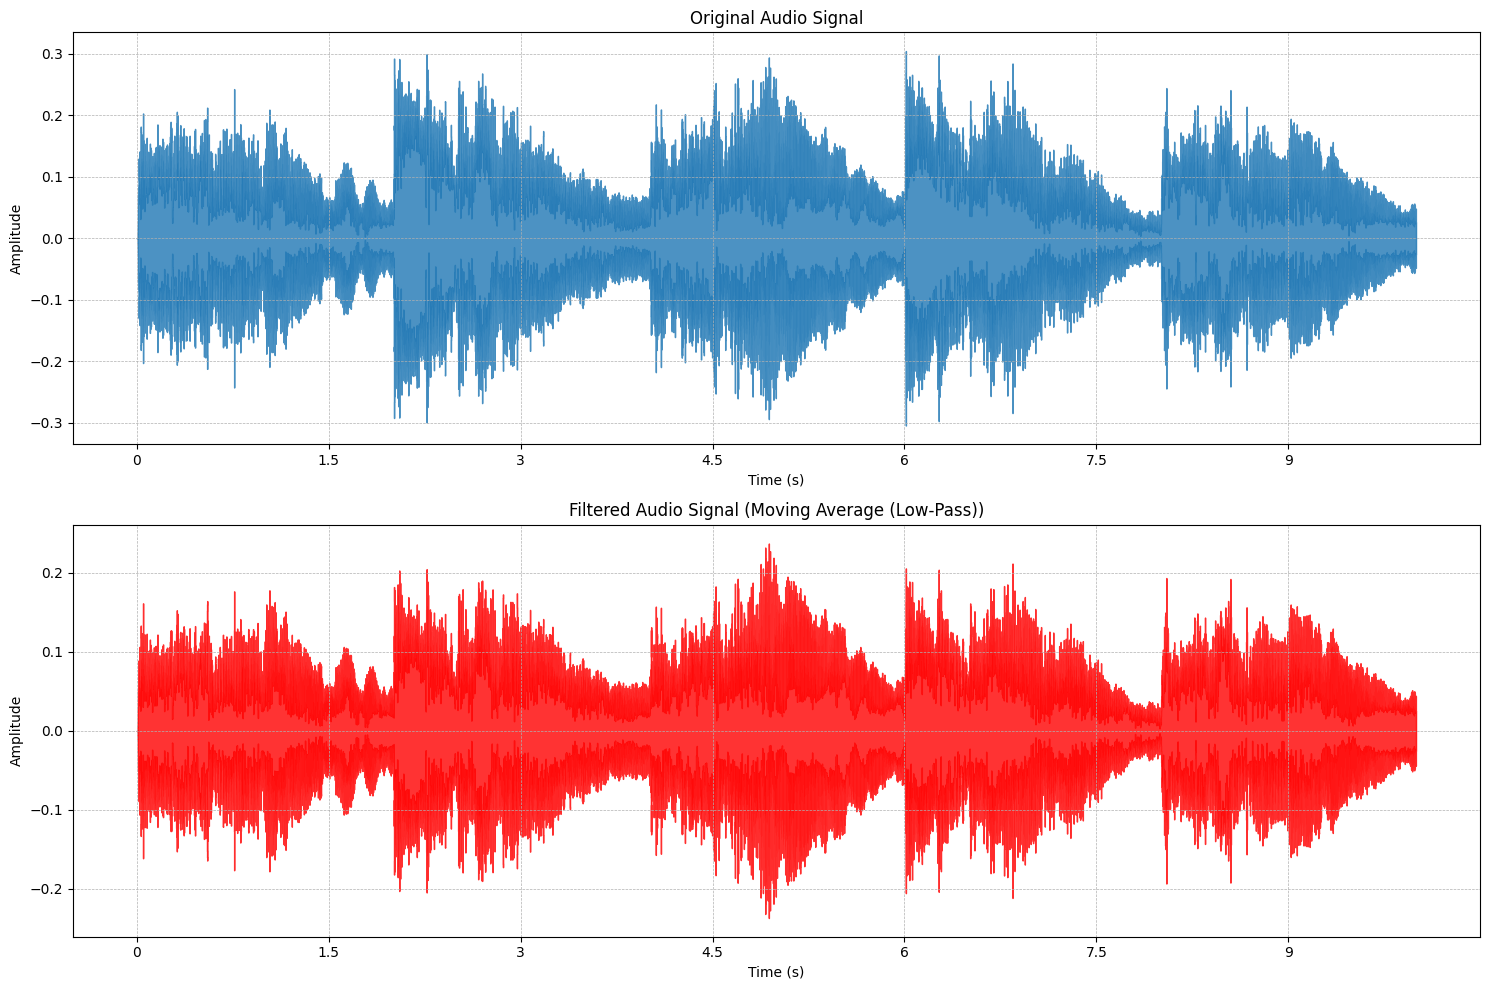
\includegraphics[width=0.9\textwidth]{Untitled(1).png} 
    \caption{Waveform of the original audio signal and filtered audio signal segment. }
    \label{fig:original_audio}
\end{figure}

\begin{figure}[H]
    \centering
    % Replace 'filtered_audio_waveform.png' with the actual filename of your plot
    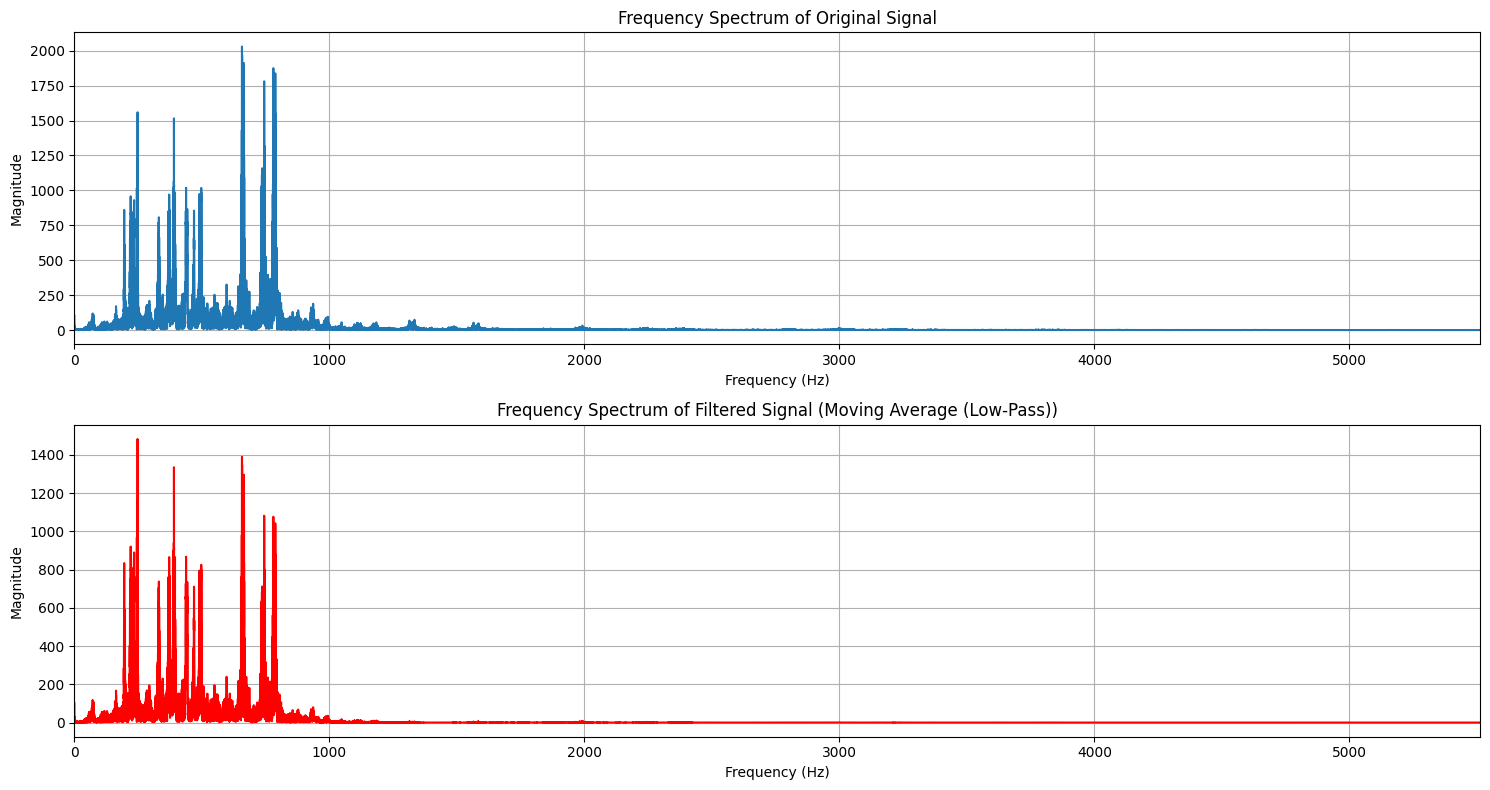
\includegraphics[width=0.9\textwidth]{Untitled.png}
    \caption{Frequency spectrum of the original audio signal and filtered audio signal segment.}
    \label{fig:filtered_audio}
\end{figure}


\subsection{Discussion of Results}

\begin{itemize}
    \item \textbf{Visual Analysis of Waveforms:}
        \begin{itemize}
            \item Comparing the original (Figure \ref{fig:original_audio}) and filtered waveforms (Figure \ref{fig:filtered_audio}), the moving average filter produced a noticeably smoother signal by attenuating rapid fluctuations and sharp transients.
        \end{itemize}

    \item \textbf{Auditory Analysis:}
        \begin{itemize}
            \item Listening to the filtered audio revealed a muffled or duller sound due to loss of high-frequency content, consistent with expectations for a low-pass filter.
            \item For median filters or noise-specific filters, the filtered audio would sound cleaner, with fewer clicks or impulsive noise.
            \item These perceptual changes align well with the filter’s theoretical effects.
        \end{itemize}
    \item \textbf{Effectiveness of the Filter:}
        \begin{itemize}
            \item The filter performed as expected, smoothing the signal and reducing unwanted high-frequency noise.
            \item Trade-offs include potential over-smoothing, which may reduce audio clarity or desired sharpness.
        \end{itemize}
\end{itemize}


\section{Conclusion}
\label{sec:conclusion}

This assignment demonstrated the use of convolution to filter an audio signal.

\begin{itemize}
    \item \textbf{Summary:} An audio signal was loaded, a moving average (low-pass) filter was applied via convolution, and the original and filtered signals were compared visually and aurally.
    \item \textbf{Key Findings:} The filter smoothed the waveform and attenuated high-frequency content, resulting in a muffled sound. Visual plots confirmed these effects.
    \item \textbf{Significance:} Convolution with different kernels can effectively modify audio characteristics, a fundamental technique in audio processing tasks like noise reduction and sound design.
    \item \textbf{Limitations:} This work used a simple filter and qualitative analysis. More complex filters and quantitative evaluation could provide deeper insights. Edge artifacts from convolution may occur near signal boundaries.
    \item \textbf{Future Work:} Possible extensions include:
        \begin{itemize}
            \item Exploring other filter types (high-pass, band-pass, IIR).
            \item Implementing fast convolution via FFT for efficiency.
            \item Designing filters for targeted effects or noise removal.
            \item Applying methods to diverse audio signals (speech, environmental sounds).
            \item Developing an interactive GUI for filtering.
        \end{itemize}
\end{itemize}

Convolution remains a versatile and powerful tool in audio signal processing, enabling a broad range of sound modifications.



% --- APPENDIX (OPTIONAL) ---
% \appendix
% \section{Supplementary Material}
% \label{app:supplementary}
% [Include any additional information, derivations, or extended code if necessary.]

\end{document}
% --- DOCUMENT END ---
